\documentclass[12pt]{article}

% House style preamble
\input{.house-style/preamble.tex}

% Update PDF metadata
\hypersetup{
  pdftitle={Effective without Warrant: Causal-Normative Networks and the Social Life of Status},
  pdfauthor={}
}
\AtBeginBibliography{\emergencystretch=3em\sloppy}

% WORKING SUBMISSION TITLE. Earlier candidates remain in planning/brief.md:
%   - What Is a Causal-Normative Network?            (blunt)
%   - Normative Status in Causal Networks            (journal-friendly)
%   - How Normative Status Enters Causal Explanation (journal-friendly)
%   - Mixed Networks: Causation, Recognition, and Deontic Status
%   - The Structure of Causal-Normative Explanation
\title{Effective without Warrant: Causal-Normative Networks and the Social Life of Status}
\author{}
\date{}

% Typed-edge network diagrams (local figure support)
\usepackage{tikz}
\usepackage{float}
\usetikzlibrary{arrows.meta, positioning}
\definecolor{xGreen}{RGB}{27,158,119}
\definecolor{xOrange}{RGB}{217,95,2}
\definecolor{xPurple}{RGB}{117,112,179}
\tikzset{
  kind/.style={draw, rounded corners, align=center, font=\small, inner sep=3pt, minimum height=9mm},
  ghost/.style={draw, rounded corners, align=center, font=\small, inner sep=3pt, minimum height=9mm,
                draw=gray, text=gray, dash pattern=on 2pt off 1.5pt},
  flagged/.style={draw, rounded corners, align=center, font=\small, inner sep=3pt, minimum height=9mm,
                draw=black, text=black, dash pattern=on 3pt off 2pt},
  causal/.style={-{Stealth}, semithick},
  ntrans/.style={-{Triangle}, semithick, xOrange},
  constit/.style={xPurple, very thick, double, double distance=1pt},
  recog/.style={-{Stealth}, semithick, dashed, xGreen},
  void/.style={gray, very thick, double, double distance=1pt, dash pattern=on 2pt off 2pt},
}
\newcommand{\edgelegend}{%
  \begin{scope}[shift={(0,-3.4)}]
    \draw[causal] (0,0) -- ++(0.9,0);    \node[right,font=\footnotesize] at (1.0,0) {causal};
    \draw[constit] (0,-0.6) -- ++(0.9,0); \node[right,font=\footnotesize] at (1.0,-0.6) {constitutive};
    \draw[ntrans] (5.2,0) -- ++(0.9,0);   \node[right,font=\footnotesize] at (6.2,0) {normative-transition};
    \draw[recog] (5.2,-0.6) -- ++(0.9,0); \node[right,font=\footnotesize] at (6.2,-0.6) {recognitional};
  \end{scope}%
}

\begin{document}
\maketitle

\begin{abstract}
Social status-assignments can support projection without moral warrant. From a promise we infer duty and claim; from release, lapse; from judgment, procedural consequences; from discriminatory standing, credibility loss, exclusion, or anticipatory adjustment. Extending \textcite{khalidi2018nodes}'s account of projectible kinds, I argue that such inferences travel through \term{causal-normative networks}: typed structures joining causal uptake, status transition, recognition, and constitutive ties within a practice or field. The payoff is an account of how status-assignments can be effective, field-stabilized, enforceable or final, recognitionally mistaken, and morally unwarranted in different combinations.
\end{abstract}

\section{The problem of mixed explanation}
\label{sec:problem}

Dickens gives the problem its comic legal form in \emph{Bardell v. Pickwick}: a misconstrued exchange becomes an action for breach of promise, then a damages verdict, and then Fleet Prison.\footnote{In \emph{The Pickwick Papers}, Mrs Bardell's action lays damages at \pounds 1,500, the jury awards \pounds 750, and Pickwick's refusal to pay carries him toward imprisonment for debt \citep[chaps.~26, 34, 40--41]{dickens1837PickwickPapers}.} Put abstractly, suppose a community or court comes to treat someone as having promised when he hasn't, or as bound by a debt he never incurred.

The treatment is not imaginary: he is asked to pay, blamed when he refuses, distrusted, perhaps shut out. But if the promise was never made, those responses lack the obligation they purport to answer to; the demand has the social force of a warranted demand without its warrant. Cases of this sort generalize: some social statuses are real in their effects without being morally warranted; some are institutionally valid, or successfully conferred by a communal practice, without being morally warranted. The problem is to explain what can be projected from such assignments, and why those projections don't settle warrant.

Identifying status with treatment makes the wrongly-hounded man indistinguishable from a genuine debtor. Treating status as only a rule-bound normative fact makes the hounding irrelevant. The case needs both pieces: a normative position, and a causal uptake that can fit that position or fail to. It also needs three families of assessment kept apart: social efficacy, institutional or communal standing, and moral warrant.

Promising is the case I work through, because its life-cycle is familiar and its parts are clean: an act creates an obligation, the obligation is recognized and relied on, breach sets off demand and repair, release cancels the profile. The same shape recurs in consent, in official judgment, and, most systematically, in discrimination, where an assignment that's effective and successfully conferred within its practice hardens into a regime that morality disowns (Section~\ref{sec:misrecognition}). I keep to promising until then.

False promise and discrimination pull the model in different directions. In the false-promise case, the status fails to obtain and recognition answers to nothing. In the discriminatory case, the standing may be genuinely conferred and real while remaining unwarranted. Promising is the clean entry case, not the template for both.

The model rests on four kinds of dependence, three of them directed edges and the fourth a non-directed constitutive tie.

First, \term{causal dependence}: one event, disposition, procedure, response, record, sanction, or expectation helps produce another. A public promise causes reliance; a judgment can cause enforcement; a recognition state causally drives treatment, and that uptake is where much of the network's efficacy lies.

Second, \term{constitutive dependence}: one deontic position is the correlative of another within a single complex. A duty and the claim-right held against the duty-bearer are one jural relation under two descriptions, so from either one reads off the other \citep{hohfeld1913SomeFundamental}. The tie is constitutive, not causal.

Third, \term{normative-transition dependence}: a performance, rule, status, or transition event generates, blocks, terminates, defeats, or modifies a status. An undertaking generates a duty; release terminates it; withdrawal terminates a permission; breach generates a secondary profile of demand, blame, apology, repair, or excuse.

Fourth, \term{recognitional dependence}: a belief, record, or official classification purports to track a status, fitting it, misfitting it, or answering to no status at all. What recognition then drives is causal uptake: demand, sanction, reliance, exclusion. Where recognition is authorized to make the status it records, as a court judgment makes an adjudicated liability, the case is compound: recognition plus transition.

These four dependence types describe the structure of the network. They don't yet say whether a status-assignment is valid. Assessment is cross-cutting: an assignment may be effective when recognition and uptake fire, \term{field-valid} when it satisfies institutional rules, successfully conferred when agents with standing in a communal practice impose constraints and enablements, and morally warranted when the standing or treatment has moral authority.

A \term{field} here is a normative practice or domain, such as ordinary promising, friendship, contract law, criminal law, or medical ethics, with its own statuses and conditions for generating them. Institutional fields fix offices, procedures, records, and rules. Communal fields fix standing relations without a single authorizing office. Section~\ref{sec:fields} treats fields as the practice-relative settings in which statuses support projections.

The network is not a replacement for grounding. It is an explanatory representation that displays, in one structure, the field-relative grounds of statuses, their correlative positions, the recognitions that fit or misfit them, and the uptake through which they become socially projectible. Epstein-style frame principles and anchors explain why the field's status conditions are in place; the network explains how those conditions combine with recognition and causal response.

\section{Why ordinary causal networks aren't enough}
\label{sec:causal-not-enough}

One tempting simplification is to treat causal-normative networks as ordinary causal networks with moral labels added. The best reason to try that comes from \textcite{khalidi2018nodes}. Khalidi takes projectibility as the mark of a kind: if something is gold, one can infer its melting point, density, conductivity, and other properties; if something is merely dirt, the label tells us much less. A kind matters for explanation when membership supports such inferences.

For Khalidi, those inferences work because the properties are ordered, not because they merely travel together. Gold's atomic structure explains many of its other properties. A directed causal graph captures that order: change one property in the right way, hold the rest fixed, and another property shifts. The functionless widget fails because its properties form a heap rather than an ordered pattern.

That point should be preserved. Projection needs order. The question is whether all useful order in the moral and institutional domain is causal order.

Promises make the limit visible. Suppose Nora promises to return a borrowed book on Friday. From the promise we can project several things: Owen has a claim, Nora owes performance, Owen may rely, breach may license demand or apology. Some of those projections are causal. Nora's words may cause Owen not to buy another copy. But the duty and the claim-right aren't cause and effect; they are the same promissory relation viewed from two sides.

Release makes the point again. If Owen releases Nora on Thursday, the same Friday non-return no longer counts as a breach. The release needn't cause the non-return, the book, or Nora's later conduct. It changes what the later non-performance amounts to. That dependence is directed, since release changes breach status and not the other way around, and it supports projection from release to the absence of liability or repair. But it isn't causal in Khalidi's sense.

Consent has the same shape. A patient signs a consent form before a procedure. The signed form may causally move many things: a nurse updates the chart, the surgeon schedules the room, the anaesthetist prepares the drugs. But the permission relation is not just that causal chain. If the patient withdraws consent before the procedure, the same incision changes status. It is no longer permitted treatment but a wrong. The withdrawal orders the later facts, because it changes what the later act is, even if some staff do not hear about it and the causal machinery keeps moving.

The extension to Khalidi is narrow. Projectibility still requires order. In moral and institutional cases, some of the order is carried by normative transitions and recognitional links rather than by causal mechanisms alone. Section~\ref{sec:typed-edge} builds that typed network; the present point is only that ordinary causal networks are too narrow, not that order was the wrong demand.

\section{Why normative taxonomies aren't enough}
\label{sec:normative-not-enough}

The opposite simplification keeps the normative structure and strips away the causal uptake. That is tempting too. Analytic jurisprudence has mapped much of the structure: \textcite{hohfeld1913SomeFundamental} sorts deontic positions into correlatives and opposites, claim and duty, power and liability. A taxonomy in this style can say that a promise generates an obligation, consent a permission, release a termination, and breach a license to complain.

That taxonomy is indispensable, but it is not yet an explanation of projection in practice. Suppose Nora fails to return the book. The taxonomy says she has breached and that Owen may complain. It doesn't say whether Owen notices, whether the complaint is taken up, whether Nora apologizes or offers an excuse, whether repair follows, or whether trust changes between them.

Those further regularities are what make promise-breaking projectible as a social kind. Breach has a recognizable place in a life-cycle: registration, demand, excuse or apology, repair or sanction, revised trust. The status starts the sequence, but the sequence runs through recognition and causal uptake.

Official judgment makes the same point in a more formal register. A taxonomy can say, in broad terms, that a judgment creates an adjudicated liability, a final or preclusive position, or a remedial profile \citep{americanLawInstitute1982RestatementJudgments}. But what makes judgment projectible in practice is also the file, the docket entry, the enforcement routine, the attorney's letter, the threat of contempt, and the debtor's changed bargaining position. Those are not further deontic implications written into the word \enquote{judgment}; they are the ordinary uptake by which a legal status becomes socially and institutionally effective.

This is why a purely normative taxonomy is too thin. A status no one could recognize, rely on, or enforce would support no social projection at all. It would still be a status, but it would not explain the patterned responses by which promise-breaking, consent withdrawal, judgment, or discriminatory ascription become stable objects of expectation.

The two reductions now fail from opposite sides. Causal order alone was too narrow; normative order alone is too thin. The explanatory unit is neither causal regularity nor normative status by itself, but a normative position coupled to causal uptake. Section~\ref{sec:misrecognition} turns to the cases in which the two come apart.

\section{The typed-edge model}
\label{sec:typed-edge}

If the explanatory unit is a normative position coupled to causal uptake, the graph has to show both parts. In the promise case it has to show the obligation and claim-right; otherwise the wrongness of demand is lost. It also has to show uptake, reliance, demand, and repair; otherwise the promise has no social life.

I keep \textcite{khalidi2018nodes}'s picture of a kind as a highly connected node in a directed graph, but I let the edges differ in type. The vertices are property instances and states; the edges are typed relations of dependence.\footnote{Formally, this is a typed-edge relational structure: node labels for kinds, edge labels for dependence types, and well-formed configurations. \textcite{pullumRogers2008Expressive} use a similar node/edge format for English syntax; the analogy only marks the intended level of abstraction. \textcite{pullum2001} set out the model-theoretic stance.}

The graph is not a new layer of metaphysics. Nora's duty is grounded by her undertaking under the rules of the relevant field; Owen's claim-right is the correlative position; Owen's reliance is an ordinary causal effect; his recognition is a representation of the duty. The network displays those relations together. It doesn't replace the grounding story. In \textcite{epstein2015AntTrap}'s terms, the field's frame principles fix the grounding conditions, while offices, records, routines, expectations, and uptake help anchor those principles.

The strongest rival is a division of labour: use grounding and anchoring to explain the status, then use causal mechanisms to explain uptake. The network adds a further claim. It represents the projection profile that crosses those explanations. From one source item it tells us which inferences run through grounds, which through correlatives, which through representation, and which through uptake. No one of the separate stories marks their interaction.

To draw such a graph, start with the explanatory question. If the question is why Owen may demand performance, the duty and claim-right matter. If the question is why Nora is shunned despite never promising, the false recognition and its causal uptake matter. If the question is why a court order leads to enforcement, the judgment and the enforcement machinery matter.

The node types are simple. Performances include utterances, signed documents, actions, and omissions. Statuses include obligation, permission, power, liability, immunity, and standing. Transition events include undertaking, authorization, release, withdrawal, breach, and defeat. Recognition states include belief, record, and official classification. Uptake and response states include reliance, demand, blame, resentment, apology, repair, sanction, exclusion, and trust revision. A field is not another node; it fixes which of these items count.

The carrying cases fill those slots in familiar ways. In a promise, the undertaking generates a duty; recognition by the promisee or audience helps drive reliance, demand, apology, repair, and trust revision. In consent, giving or withdrawing consent changes a permission profile, while recognition determines whether others proceed, stop, complain, or apologize. In a judgment, the court's act is both an official recognition and a status-altering event, with records, enforcement, and remedies downstream. In discrimination, a signal or classification drives uptake, and stabilized uptake can help confer a degraded standing.

Consider the promise graph as a drawing exercise. Nora's utterance goes in because it can generate the duty and cause reliance. The duty goes in because it is what Owen's demand purports to answer to. Owen's uptake goes in because demand and repair usually pass through his recognition of the promise. The weather, Nora's mood, and the room's acoustics stay out unless they matter to the explanatory question. If the question is only why Owen relied, acoustics may matter; if the question is whether Nora owed performance, they usually do not.

Now change the case. Suppose Nora never promised, but Owen misheard a joke as an undertaking. The graph should not silently insert a duty node to make sense of Owen's anger. It should show Owen's recognition state and its causal downstream: demand, blame, distrust. The absent duty is part of the explanation, because it is why the demand misfires. A purely causal graph would see only Owen's anger; a purely normative taxonomy would see only the absence of duty. The mixed graph shows both.

The admission rule is practical: add a node only if leaving it out would make the explanation worse. A performance enters when it can generate, alter, defeat, or causally move a status, recognition, or response. A status enters when the field's conditions make it obtain. If the dispute is whether the status obtains, as with Pickwick's alleged promise, the graph may mark the candidate as absent rather than draw it as an ordinary status node.

The same discipline applies to edges. Draw a causal edge only where one item helps produce another. Draw a normative-transition edge only where a performance, rule, status, or transition event generates, terminates, blocks, defeats, or modifies a status. Draw a constitutive tie only where two positions are one relation under two descriptions. Draw a recognitional edge only where recognition fits an actual status node.

That last rule matters. In a false-promise case, demand doesn't prove a duty. The graph should show a recognition node with live causal uptake and no fitting recognitional edge to an actual duty. Nor should moral warrant appear as a further status node that causes legitimacy; warrant is an assessment of the assignment. And the duty--claim-right tie should not be replaced with a causal arrow, since correlatives are not two states linked by a mechanism.

The network's four dependence types fall into three directed edges, causal, normative-transition, and recognitional, and the non-directed constitutive ties among deontic correlatives. Two further notions sit just outside the inventory. \emph{Authorized recognition} is the judgment case: a court records a liability and, because the field authorizes the court to do so, creates a new procedural status. \emph{Projection} is what the graph is for: using one point in the network to make defeasible inferences about what else should hold or what will happen next.

The edge types are told apart by their behaviour under intervention or analogous counterfactual probes, reserving \emph{intervention} in the strict Woodwardian sense for causal edges. \textcite{woodward2003MakingThingsHappen} counts a relation as causal when some possible intervention on the first variable changes the second while everything else is held fixed, and the change reaches the second only through the first \citep{woodward2014MethodologyOntology}.

A causal edge passes this test in the ordinary way: intervene on the utterance and reliance shifts, intervene on the judgment and enforcement may follow. Khalidi already reads his own causal edges this way \citep{khalidi2018nodes}, which is why typing the edges extends his picture rather than breaking with it.

A constitutive tie fails the test in a way that helps mark its type. A duty and its correlative claim-right aren't two states linked by a mechanism; they're one jural relation under two descriptions \citep{hohfeld1913SomeFundamental}. No intervention changes the duty while holding the claim-right fixed, because changing the one just is changing the other: the change doesn't reach the claim-right only through the duty, it lands on both at once. By Woodward's own criterion the tie isn't causal, and that failure is what marks it as constitutive.

The transition and recognitional edges are directed without being causal. A normative-transition edge runs from a performance, rule, status, or transition event to the status it generates, terminates, blocks, defeats, or modifies: release the promisor and the same non-performance is no longer a breach.

A recognitional edge connects an actual status node to a recognition node that fits it. A belief, record, or classification, itself driven by signals and cues along causal edges, may also misfit or answer to no status at all. In those failed cases the recognition node remains, with its outgoing causal edges, but the fitting recognitional edge is absent or failed. That gap is what the \enquote{mis-} in misrecognition marks.

One occurrence can also enter more than one relation. The same utterance \enquote{I'll do it} may causally induce reliance, generate a duty if made under the right conditions, and become the object of later recognition. The same court order can be evidence in one setting, an operative change in another, and the cause of enforcement in a third. A racialized name on a resume is different again: it is not the status it signals, but a cue that causally moves recognition, which then moves callback behavior.

When representation succeeds the recognition tracks its status (Figure~\ref{fig:promise}); whether it fits is separate from what it sets off, since the uptake to treatment, demand, sanction, reliance, exclusion is causal, the point where the normative layer re-enters the causal one.

An illocutionary act, in \textcite{sbisa2023OnIllocutionaryTypes}'s terms, assigns or cancels deontic-modal predicates, and so appears here as a performance feeding a normative-transition edge.

Figure~\ref{fig:promise} renders a promise as a small network of this kind, with the four edge types that recur across the carrying cases.

\begin{figure}[tb]
  \centering
  \resizebox{\textwidth}{!}{%
  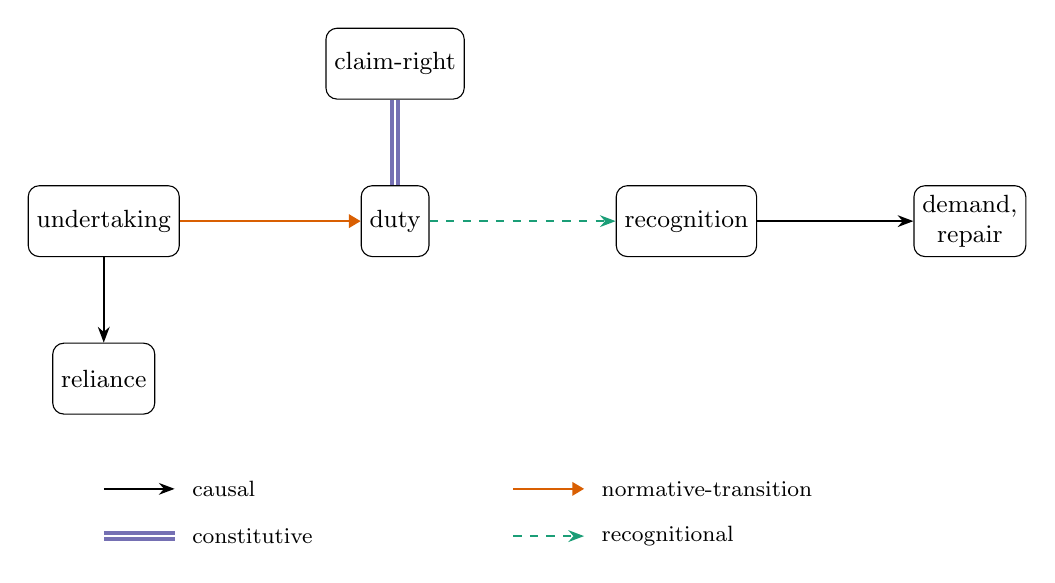
\begin{tikzpicture}
    \node[kind] (u) at (0,0)    {undertaking};
    \node[kind] (o) at (3.7,0)  {duty};
    \node[kind] (k) at (3.7,2)  {claim-right};
    \node[kind] (r) at (7.4,0)  {recognition};
    \node[kind] (d) at (11.0,0) {demand,\\repair};
    \node[kind] (l) at (0,-2)   {reliance};
    \draw[ntrans]  (u) -- (o);
    \draw[recog]   (o) -- (r);
    \draw[causal]  (r) -- (d);
    \draw[constit] (o) -- (k);
    \draw[causal]  (u) -- (l);
    \edgelegend
  \end{tikzpicture}}
  \caption{A promise as a causal-normative network. The undertaking generates the duty (a normative transition) and causally induces reliance; the duty carries its correlative claim-right (a constitutive tie, drawn without an arrowhead, since correlatives are one relation under two descriptions, not a directed cause); the duty is tracked by recognition, which causally drives demand and repair (the recognitional arrow is drawn in the fitting case; in failed cases the recognition node remains without a fitting edge, Section~\ref{sec:typed-edge}). The four edge types are keyed below the graph.}
  \label{fig:promise}
\end{figure}

Two conditions keep such a graph from sliding back into a mere list of properties. First, inference has to respect edge type. The projection ledger is mixed: causal edges license predictions of uptake or response; constitutive ties license read-offs from one deontic position to its correlative; normative-transition edges license projections from performances or rules to generated, defeated, or altered statuses; recognitional edges license expectations about tracking, misfitting, and downstream uptake.

Second, a status that is meant to explain a social cascade has to be reachable by response states through recognition and causal uptake. A status can obtain without being noticed, but it explains projectible demand, enforcement, apology, exclusion, or repair only where the field supplies pathways by which agents can track or respond to it.

Table~\ref{tab:projection-ledger} gives the compact ledger for the four carrying cases. It is not a list of case outcomes; it is a guide to what kind of inference each source item supports, and where that inference can fail.

\begin{table}[H]
\centering
\small
\setlength{\tabcolsep}{3pt}
\begin{tabular}{@{}>{\raggedright\arraybackslash}p{0.15\textwidth}>{\raggedright\arraybackslash}p{0.16\textwidth}>{\raggedright\arraybackslash}p{0.16\textwidth}>{\raggedright\arraybackslash}p{0.25\textwidth}>{\raggedright\arraybackslash}p{0.18\textwidth}@{}}
\toprule
Case and field & Source item & Main edge & Projection & Defeater or limit \\
\midrule
Promise, ordinary promising & Undertaking & Normative-transition; constitutive & Duty and correlative claim-right; reliance, demand, apology, or repair if recognized & Joke, coercion, release, or lack of standing \\
Consent, medical ethics & Consent or withdrawal & Normative-transition; recognition-to-uptake & Permission, its lapse, charting, stopping, complaint, or apology & Incapacity, defective disclosure, withdrawal, emergency, or missed recognition \\
Judgment, law & Court judgment & Authorized recognition: recognition plus transition & Adjudicated status, record, finality or preclusion, remedial and enforcement profile \citep{americanLawInstitute1982RestatementJudgments} & Lack of jurisdiction, appeal, vacatur, procedural defect, or moral error \\
Discrimination, communal practice & Signal or ascription plus standing uptake & Causal recognition path; communal conferral & Lowered credibility, restricted options, risk, routing, anticipatory adjustment & Weak uptake, counter-practice, lack of standing, or no durable position \\
\bottomrule
\end{tabular}
\caption{A compact projection ledger. Each row gives the field, the source item from which projection starts, the main edge type, the target of projection, and the defeaters or limits that keep projection from becoming moral warrant.}
\label{tab:projection-ledger}
\end{table}

With those conditions in place the graph carries order in Khalidi's sense, projection along directed edges, while generalizing what that order is: not causal dependence throughout, but directed dependence of three kinds, causal, normative-transition, and recognitional, running within constitutive constraints.

All these nodes and edges are field-indexed: which performances count, which recognitions are authoritative, and which responses are licensed depends on the field, to which Section~\ref{sec:fields} returns.

\section{Coupling and counterfactual signatures}
\label{sec:coupling}

The easiest way to see the coupling is to ask simple what-if questions. What if Owen releases Nora? What if Owen mistakenly believes Nora promised? What if a court enters judgment? Each change moves a different part of the graph, and the pattern tells us which kind of edge is doing the work. I call these patterns \emph{signatures}. I reserve \emph{intervention} for the genuinely causal edges, where Woodward's apparatus applies directly.

The first what-if changes a status or the rule behind it. Release the promisor and later non-performance is no longer a breach; the demand, blame, and repair that breach would license lapse with it. Withdraw consent and the same act of touching changes from permitted to wrongful. Speak without standing and the same words fail to bind; an official's words and a bystander's words don't have the same status effects. These are the status-altering acts the normative-powers literature describes \citep{owens2012ShapingNormativeLandscape,raz2022NormativePowers}.

Call that a \term{status-rule signature}. The status node changes first in the order of explanation, and uptake follows because agents now have a different status to recognize or answer to. The audience may be psychologically unchanged at the first moment: Owen may still expect the book, the doctor may still prepare the procedure, the clerk may still open the file. What has changed is what their responses would now be responses to. The signature licenses projection from release, withdrawal, or authorization to changed duty, permission, liability, or remedial profile even when uptake lags.

The consent example is useful because the surface behavior can remain almost unchanged. A clinician reaches for the same instrument, at the same time, for the same medical reason. Before withdrawal, that act is within the permission profile. After withdrawal, the same act of touching is no longer licensed. If the clinician has not heard the withdrawal, her recognition node may still represent the old permission, and her action may continue along the old causal path. The status-rule signature and the recognition signature come apart in one ordinary case.

The second what-if changes recognition while the status stays put. Suppose Nora never promised, but Owen and the audience believe she did. There is no promise-duty node for recognition to fit, but the false recognition node can still drive demand, blame, and loss of trust. Suppose consent has been withdrawn but the withdrawal is not registered. The permission profile has changed, but the old response path may keep running.

Call this a \term{recognition signature}. The recognition node may fit the status, misfit it, or answer to no status at all. Either way, the causal edge leaving the recognition node can fire. In hiring, changing the employer's belief about an applicant's gender changes the recognition node and the causal edge from recognition to callback while leaving the applicant and the moral facts unchanged. Woodward's own reading of \enquote{being a woman causes hiring discrimination} relocates the cause to the employer's beliefs about the applicant's gender \citep{woodward2014MethodologyOntology}: a recognition signature in the present sense, projecting efficacy without projecting warrant.

The third what-if is the compound case. A judgment records, finds, or accepts a status, but the field also gives that act a power to change the status profile. Before judgment, the alleged liability may be disputed. After judgment, the field may treat the parties as occupying a new procedural or remedial position even where the court is mistaken: a record, enforceability, finality or preclusion, or remedial power \citep{americanLawInstitute1982RestatementJudgments}. A release in contract law can likewise terminate the obligation profile even if demand continues \citep{americanLawInstitute1981RestatementContracts}.

This is \term{authorized recognition}. It is not a fifth primitive. The same node occupies two roles: recognition, because it records or finds; transition, because the field authorizes that recognition to make a status difference. The signature projects field-valid procedural consequences from the authorized act without projecting moral warrant or truth of the underlying finding.

Pickwick again shows why the compound matters. The alleged proposal does not by itself create the promised obligation. But the verdict creates an adjudicated liability within the procedure of the court. That position can be entered in a record, treated as settled for procedural purposes, and routed into remedial or enforcement machinery. One mistake is to say that the judgment merely recognizes a liability already there. Another is to say that the judgment is just a cause of imprisonment. It is both recognition and status transition: a finding that the field treats as operative.

These signatures depend on a separability assumption. We have to be able, at least in explanation, to change one node or edge while holding the adjacent structure fixed. Woodward calls this \term{modularity}: mechanisms are separately disruptable in principle \citep{woodward2003MakingThingsHappen}. The condition is not trivial. In an actual field, rules, records, and uptake often move together, which is why the signatures are explanatory probes rather than field experiments.

Constitutive ties fail that separability condition. One can't change a duty while holding the correlative claim-right fixed, since the two are one relation under two descriptions. The status-rule and recognition contrasts pass. Release the promisor and the obligation lapses while the audience's belief can remain; change an employer's belief while the applicant's status remains. Modularity sorts the edge types rather than flattening them.

I set aside a pure causal intervention, such as severing an uptake mechanism so the letter never arrives, because both reductive views already grant it. It can't tell the reductive views apart from the coupled account.

The status-rule and recognition signatures expose the mistake in the forced choice. The recognition reduction predicts that enough uptake turns the recognition node into the status node. The normative reduction keeps the status node but treats misfiring recognition and its causal effects as noise. False promise shows why both are wrong: demand may be real without a duty, and the absence of duty still matters.

The point carries across the cases. A causal graph with moral labels can't explain release, because labels don't change breach status. A normative taxonomy with sociology appended can't explain false uptake, because it has nowhere to put efficacy without warrant. The coupled, typed structure is needed because it predicts which part of the case moves and which part holds fixed.

An interventionist objection presses from the other direction. Why not drop the network label and disambiguate everything into manipulations of beliefs, records, and behavior? The reply turns on Woodward's own view that interventionism is methodology, not ontology \citep{woodward2014MethodologyOntology}. It clarifies causal claims by tying them to hypothetical experiments; it doesn't say that every relation clarified in that way is causal.

The promise case shows the difference. Release the promisor and the obligation node lapses, even if the audience keeps believing that the promisor owes performance. Change the audience's belief instead, and demand or blame may move while the duty does not. Both probes need the status node: without it, one can record who demanded what, but not whether the demand fitted an obligation.

The same point holds for discrimination. If a correspondence study changes the employer's belief, it identifies a causal path from signal to recognition to callback. It doesn't settle whether the belief fits the applicant's social status, or whether the status assignment has warrant. The interventionist disambiguation is useful, but it marks rather than removes the place where a normative edge is needed.

\section{Misrecognition as the diagnostic case}
\label{sec:misrecognition}

Misrecognition is the sharpest diagnostic because it asks a plain question: what should we say when people treat someone as bound, liable, authorized, dangerous, or disqualified, and that treatment is wrong? A recognition-only account says the treatment makes the status. A purely normative account says the treatment is noise around the real status. Neither answer fits Pickwick, who is effectively hounded as a promisor without having made the promise.

The network separates four questions. Is the assignment socially effective? That is a question about uptake: do people rely, demand, enforce, exclude, record, or sanction? Is it institutionally field-valid? That is a question about the right party, office, procedure, form, record, rule, or authority. Is it successfully conferred in a communal practice? That is a question about standing in context and imposed constraints and enablements. Is it morally warranted? That is a question about whether the standing or treatment has moral authority rather than imposing unjust constraint.

Table~\ref{tab:assessment} turns those questions into a checklist for status-assignments. Some columns are basic families of assessment; others are refinements needed for institutional, procedural, and recognitional cases. They often travel together in ordinary cases, but none carries the others with it.

\begin{table}[H]
\centering
\small
\setlength{\tabcolsep}{3pt}
\begin{tabular}{@{}>{\raggedright\arraybackslash}p{0.22\textwidth}>{\raggedright\arraybackslash}p{0.43\textwidth}>{\raggedright\arraybackslash}p{0.25\textwidth}@{}}
\toprule
Assessment & Question & Does not settle \\
\midrule
Social efficacy & Do recognition and uptake produce reliance, demand, enforcement, exclusion, records, or sanction? & Whether the status obtains or is warranted \\
Institutional field-validity & Did the right office, procedure, form, record, rule, or authority assign the status? & Truth, justice, or current recognition \\
Communal successful conferral & Did agents with standing in context place someone under constraints and enablements? & Moral authority or institutional legality \\
Recognitional fit & Does the belief, record, or classification track the status, base, or finding it purports to track? & Efficacy, validity, or warrant \\
Enforceability or finality & Can the field's machinery act on the assignment, or treat it as settled for procedural purposes? & Moral warrant or underlying truth \\
Moral warrant & Does the standing or treatment have moral authority and avoid unjust constraint? & Social efficacy or field-validity \\
\bottomrule
\end{tabular}
\caption{Assessment columns for status-assignments. The columns often travel together, but none entails the others.}
\label{tab:assessment}
\end{table}

In a straightforward case, the columns line up. A genuine promise may be recognized, valid in the relevant practice, and morally binding. But the columns can also come apart. A crowd may demand performance where no promise was made. A court may impose an adjudicated liability by a valid procedure on a mistaken record. An unjust practice may successfully confer a standing while morality rejects the standing itself.

It helps to keep the columns separate. In the false-promise case, social efficacy is present if people demand and blame, but field-validity and moral warrant are absent if no undertaking occurred. In the mistaken-judgment case, efficacy is present and legal field-validity may also be present, even though the underlying finding is wrong. In the discrimination case, a community may confer a degraded standing that is socially real and field-stabilized, while the moral-warrant column remains empty.

This gives four failure profiles. In \emph{false recognition}, uptake occurs although the assignment is neither field-valid nor morally warranted. Pickwick's alleged promise is the comic case. In \emph{wrongful institutional validity}, a field's rules assign a status while moral warrant is absent. In \emph{wrongful communal conferral}, agents with social standing impose a real standing without moral authority. In \emph{suppressed entitlement}, the moral basis is present but the field refuses recognition, as when a person has a claim that the institution declines to register.

Pickwick is useful because it keeps the first failure profile clean. Until judgment enters, there is no promised obligation for recognition to fit. The verdict then changes the case: it is an authorized recognition that creates a new legal liability. The episode shows efficacy without the promised obligation, but it does not yet show the regime structure of wrongful conferral.

Regime cases require more than one mistaken uptake. A person wrongly believed to have promised faces a local failure: demand, blame, and distrust may be real, but the error can in principle be corrected by showing that no promise was made. A durable discriminatory practice is different. It repeats the ascription, routes it through records and expectations, and gives people real constraints and enablements under that description.

Ásta's conferralist account helps specify that second structure. A social status is conferred on a person because agents with standing in a context take them to have some base property, whether or not they actually have it, and impose real constraints and enablements on what they may do \citep{asta2018Categories}. The ascribed standing is not a mere belief. It is a social position with teeth.

Conferralism might seem to collapse the distinction I need. If the status just is what gets conferred, then enough recognition constitutes the status. But the collapse is avoided once the assessment questions are separated. Conferral can make a communal status real and effective without making it morally warranted. A discriminatory standing can be genuinely conferred, field-stabilized, and morally indefensible at the same time.

Some oppression works through this route: morally indefensible status-ascriptions become socially effective, and sometimes institutionally valid or successfully conferred, along durable recognition and response pathways. Not all oppression does. Much is material, distributive, or coercive rather than recognitional, the pressure the redistribution-versus-recognition debate brings to bear \citep{fraserHonneth2003Redistribution}. Stabilized wrongful conferral is only the case this account is built to diagnose.

Material and distributive structures are not therefore invisible to the network. They can enter as causal constraints, resources, built environments, or enforcement routines. What the present section adds is narrower: when those pathways also impose a standing, the explanation needs a status node as well as causal paths to harm.

\begin{figure}[tb]
  \centering
  \resizebox{\textwidth}{!}{%
  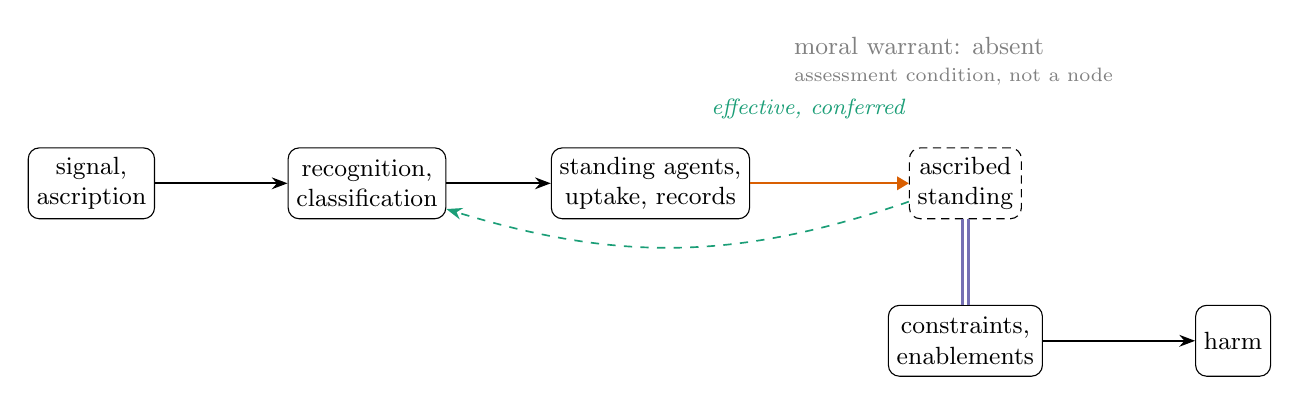
\begin{tikzpicture}
    \node[kind]    (u) at (0,0)    {signal,\\ascription};
    \node[kind]    (r) at (3.5,0)  {recognition,\\classification};
    \node[kind]    (p) at (7.1,0)  {standing agents,\\uptake, records};
    \node[flagged] (s) at (11.1,0) {ascribed\\standing};
    \node[kind]    (c) at (11.1,-2) {constraints,\\enablements};
    \node[kind]    (h) at (14.5,-2) {harm};
    \node[font=\small, align=left, text=gray, anchor=west] at (8.8,1.55)
      {moral warrant: absent\\[-1pt]\scriptsize assessment condition, not a node};
    \draw[causal] (u) -- (r);
    \draw[causal] (r) -- (p);
    \draw[ntrans] (p) -- (s);
    \draw[constit] (s) -- (c);
    \draw[causal] (c) -- (h);
    \draw[recog]  (s) to[bend left=18] (r);
    \node[font=\footnotesize\itshape, xGreen, anchor=south] at (9.1,0.7) {effective, conferred};
  \end{tikzpicture}}
  \caption{Wrongful conferral. A signal or ascription moves recognition and uptake. When agents with standing stabilize uptake through records, expectations, and response routines, they can help confer an ascribed standing whose content is a set of constraints and enablements. Later recognition may track that standing, but moral warrant is absent (grey annotation). This is not the false-promise case, where recognition fails to fit an absent status. Edge styles as in Figure~\ref{fig:promise}.}
  \label{fig:misrecognition}
\end{figure}

Read Figure~\ref{fig:misrecognition} from left to right. A signal or ascription moves recognition, and recognition moves uptake. When uptake becomes a durable practice of records, expectations, sanctions, and anticipatory adjustment, it can help confer a standing. The standing is constituted by constraints and enablements, which project altered options, credibility, risk, authority, access, self-regulation, and downstream harm.

The conferring agents are those whose uptake is structurally empowered in that context: gatekeepers, officials, employers, teachers, clinicians, peers, or a dominant local audience. The base or ascription is the property they take the person to have. The conferred status is a role-like standing in that setting rather than the base property itself: lowered credibility, suspected dangerousness, reduced authority, or disfavoured applicant standing.

Discrimination, where it runs through conferred standing, is that regime case. The efficacy is measurable, if crudely. In the correspondence study by \textcite[997--998]{bertrandMullainathan2004EmilyGreg}, otherwise-matched resumes with White-sounding names drew about 50\% more callbacks than those with African-American-sounding names (9.65\% against 6.45\%), and \textcite{ayres1991FairDriving} found parallel differential treatment in retail car negotiations. These studies evidence a signal-recognition-response pathway; they do not by themselves establish a degraded standing.

These studies show patterned uptake. A name or other raced signifier sends a causal edge to a recognition node, and that recognition node sends causal edges to callbacks, prices, warnings, searches, or other outcomes. A normative taxonomy with no place for this efficacy can't describe what's happening.

The studies do not manipulate race itself. As \textcite{weinbergerSignalManipulation} observes, they manipulate a \emph{signal} for race: the name matters because it reliably tracks race, and the experiment varies the signal to mimic what it would be were the candidate of another race, leaving the candidate's race untouched. That is a localized causal test of the signal-recognition-response pathway. It does not make race an ordinary manipulable cause, and it does not reduce race to its signals.

Detection is still not an account of discrimination. \textcite{kohlerHausmann2019EddieMurphy} is right that a signal test can show race made a difference without saying what race is or why discriminating on it is wrong. \textcite{huForthcomingNormativeFactsCausalStructure} presses further: deciding which differences between two candidates constitute rather than confound the effect of race already takes a normative stand, so even the measurement presupposes the normative layer.

What turns biased uptake into conferred standing is entrenchment under agents with social standing in that context. A single misfiring is false recognition. A stable recognition-response pathway is different. When the pathway is repeated, recorded, expected, and treated as a guide for action, it shapes what one may do, where, with what credibility, and at what risk. That imposed structure, not the bare frequency of mistreatment, is the degraded standing \citep{asta2018Categories}.

The contrast is between an episode and a position. A single employer's biased callback decision is an episode of differential treatment. It may be wrongful, and it may reveal a causal pathway from signal to recognition to response. A standing emerges when decisions of that sort become mutually reinforcing: employers expect other employers to read the signal the same way, applicants adjust their applications in anticipation, institutions record and route outcomes accordingly, and the burden becomes part of what one has to navigate. The graph then has a stable ascribed-standing node, not just repeated arrows from signal to harm.

The discrimination this account captures is entrenched wrongful conferral: recognitional and causal edges firing reliably enough to be projectible, fixing a degraded standing that the field's standing relations may sustain but morality doesn't. Other discrimination need not run through conferred standing. Resource allocation, exclusionary design, and statistical sorting can wrong without conferring a degraded status. The present account claims only the conferral-based cases.

The route to wrongful conferral begins with the recognition signature of Section~\ref{sec:coupling}. At the audit-study stage, one can vary a signal or recognition node and watch uptake move while the applicant and moral facts hold fixed. But wrongful conferral adds a further step. Once that recognition-response pathway is entrenched in a stable practice, it helps generate a degraded standing rather than merely misrecognizing one. Only a coupled, typed structure registers both moments: the recognition is real and effective, and the standing it helps stabilize remains unwarranted.

\section{Fields}
\label{sec:fields}

A field tells the graph what counts. I use \term{field} in a modest sense, for a normative practice or domain such as contract law, criminal law, medical ethics, ordinary promising, or friendship. In contract law it tells us which words, signatures, consideration, defects, and releases generate or defeat liability \citep{americanLawInstitute1981RestatementContracts}. In medicine it tells us who may consent, who may diagnose, which records count, and which responses follow. In friendship it tells us when a betrayal licenses resentment, apology, repair, or distrust.

The same surface event can receive different treatment across fields. Saying \enquote{I promise} at dinner may create an interpersonal obligation; saying the same words in a negotiation may be legally idle without the right form or consideration; saying them as part of a joke may create no obligation at all. A signature on a consent form may authorize treatment in a clinic, but a similar signature on a petition does not. The field supplies the relevant repertoire of statuses and the rules for moving among them.

Projectibility is field-relative in this sense. A status supports the projections licensed by the practice in which it figures. Breach in contract law projects toward liability, remedies, defenses, and excuses; breach in friendship projects toward resentment, apology, repair, and trust revision. Consent in medical ethics projects toward permission, disclosure duties, withdrawal conditions, and recordkeeping. Discriminatory standing projects toward lowered credibility, restricted options, sanction risk, anticipatory adjustment, and institutional routing. That is close to \textcite{boyd1999}'s accommodation thought: classifications earn their keep by helping a practice make the inferences it needs, not by having sharp boundaries independent of every practice.

In Epstein's terms, each field has frame principles that fix grounding conditions for its status facts, and anchors that explain why those frame principles are in place \citep{epstein2015AntTrap}. Applied here, the field fixes which performances ground which statuses, which records preserve them, which recognitions can alter them, and which defeaters block them.

Those conditions do not hang together by accident. Records, registers, monitoring, enforcement routines, reputational sanction, professional training, and habituated uptake help anchor and stabilize them. A field needn't itself be a natural kind or a further node in the network. For present purposes, stability means recurrence across cases, recognized routes for record or uptake, socially intelligible defeaters, and enough continuity that source nodes license defeasible expectations about target statuses and responses.

Field-validity is not the same as current recognition, enforceability, finality, or moral warrant. A contract can be valid even if a particular audience misses it; a release can terminate an obligation even if the promisee still demands performance; an unjust judgment can be procedurally valid while morally defective. The field fixes the conditions; recognition is one route by which agents track or fail to track them.

A limited analogy comes from assessment. \textcite{messick1995Validity} argues that validity attaches to supported interpretations and actions based on scores, not to an instrument considered in isolation. The present issue is practice-relative status validity, not measurement validity.

Communal cases need a further caution. In friendship, workplace standing, or discriminatory social position, there may be no office or rulebook that settles validity. The stricter question is whether the standing has been successfully conferred: whether agents with standing in that context, operating through a stable enough practice, have imposed real constraints and enablements. That can make the status socially real without making it morally warranted.

This also explains why fields can be fuzzy or contested without becoming useless. A counter-practice may reject an official rule without leaving the domain altogether. Oppressive and resistant uptake can coexist in the same workplace, clinic, court, or community. The question is whether a stable enough practice fixes the status conditions relevant to the projection at issue.

This is why the field parameterizes the network rather than sitting inside it as another node. It fixes the repertoire of statuses, the performances that generate them, the authorities that may alter them, the records that preserve them, the recognitions that count, the responses that are licensed, and the defeats that block or end them.

Field-parameterization lets the account steer between universalism and relativism: one shared typed network, many field-specific parameterizations. I use \enquote{field} for a normative practice or domain, not in Bourdieu's technical sense. The paper uses a modest point, not a general sociology of fields: status facts are assessed only relative to a practice whose status conditions are stable enough to support projection.

Fields come in at least two kinds. Institutional fields assign status functions by authorized conferral; \textcite{searle1995Construction} builds these from the assignment of function, collective intentionality, and constitutive rules. A contract, diagnosis, judgment, or accepted resignation lives here, and so does authorized recognition. Speech-act practice also belongs here when an illocutionary act alters the deontic-modal position of participants \citep{sbisa2023OnIllocutionaryTypes}.

Communal fields work differently. \textcite{asta2018Categories} marks out statuses conferred by a community with the standing to confer but by no single office, gender and race among them. That distinction explains why official judgment and discrimination, though both turn on recognition, behave so differently. The first is institutional: a recognition the field authorizes to make the status it records. The second is communal: a diffuse conferral with real constraints and enablements but no authorizing office, which is just why agents may have social standing to confer a status while lacking moral authority to do so.

\section{Conclusion}
\label{sec:conclusion}

The paper began with cases in which a person is treated as occupying a status he does not have, or is assigned a standing that a practice successfully confers while morality rejects it. A causal graph can track the hounding, sanction, or exclusion. It cannot by itself say why the treatment fails to fit. A normative taxonomy can state the duty, permission, or standing. It cannot by itself explain which social cascade that status will support.

The point is not to abandon Khalidi's causal-network account of kinds. Khalidi was right that projection needs order, not concatenation. The moral and institutional cases show that the order can be carried by non-causal edges and still support projection. A causal-normative network is the profile, stabilized by field practices, that makes the status usable for inference.

A causal-normative network lets us project different things from the same assignment. From a release we project the lapse of obligation, even if demand continues. From a judgment we project records, enforceability, finality or preclusive effects, and remedial powers, while leaving truth and warrant open. From a discriminatory standing we project credibility loss, constrained options, sanction risk, institutional routing, and self-adjustment, while withholding moral warrant.

The framework does more than remind us that some explanations contain both causal and normative material. Its stronger claim is that some projections are unavailable unless causal uptake, normative transition, recognition, and constitutive ties are represented together. That is why false recognition, wrongful institutional validity, wrongful communal conferral, and suppressed entitlement can be compared without flattening their fields.


\newpage
\printbibliography

\end{document}
